\documentclass{./../div_teaching_slides}

\begin{document}
\title{ECON 340 \\ Economic Research Methods}
\author{Div Bhagia}
\date{Lecture 17 \\ Inference in Regression Models}

%%%%%%%%%%%% 
\begin{frame}[noframenumbering, plain]
\maketitle
\end{frame}


%%%%%%%%%%%% 
\begin{frame}{Assumptions for Causal Inference}
\textit{Assumption 1 (Linearity):}
The relationship between $X$ and $Y$ is given by: 
$$ Y = \beta_0 + \beta_1 X + u $$
\vspace{1em}
$u$ is the mean zero error term, $E(u)=0$. \\~\\
\textit{Assumption 2 (Random Sample):} The observed data $(Y_i, X_i)$ for $i=1,2,...,n$ represent a random sample of size $n$ from the above population model. 
\end{frame}

%%%%%%%%%%%% 
\begin{frame}{Assumptions for Causal Inference}
\vspace{0.5cm}
\textit{Assumption 3 (No large outliers)}: Fourth moments (or Kurtosis) of $X$ and $Y$ are finite. \\~\\
\textit{Assumption 4 (\textit{Mean Independence}/Exogeneity):} The expected value of the error term is the same conditional on any value of the explanatory variable.
$$ E(u|X)=E(u)=0 $$ 
\end{frame}

%%%%%%%%%%%% 
\begin{frame}{When the exogeneity assumption fails}
$$ Y = \beta_0 + \beta_1 X + u $$ \\ \vspace{0.5em}
\begin{witemize}
\item $Y$: test scores, $X$: class-size, $u:$ teacher quality
 \item If schools with higher student-teacher ratios have worse teachers ($ \uparrow X, \downarrow u$)
 \item Then, if we see test scores decline with class size ($ \uparrow X, \downarrow Y$), hard to say if it's due to teacher quality or class size.
\end{witemize}
\end{frame}

%%%%%%%%%%%% 
\begin{frame}{Sampling Distribution for OLS Estimators}
Under Assumptions 1-4, in large samples ($n>100$), 
 $$ \hat{\beta_0} \sim N(\beta_0, \sigma^2_{\hat{\beta_0}}), \quad \quad  \hat{\beta_1} \sim N(\beta_1, \sigma^2_{\hat{\beta_1}}) $$
 
 where $$ \sigma^2_{\hat{\beta}_1} = \frac{1}{n} \frac{Var[(X_i-\mu_X)u_i]}{Var(X_i)} $$	
\end{frame}

%%%%%%%%%%%%
\begin{frame}{Test Scores and Class Size}
We estimated the following model:
$$ Test Score_i = \beta_0 + \beta_1 \cdot STR_i + u $$
And found:
$$ \hat{\beta_0} =698.93 \quad \text{and} \quad \hat{\beta_1}=-2.28   $$ \\
\vspace{1em}
Even if $E(u|STR)=0$, some uncertainty around estimates due to sampling variation. Do we really know whether -2.28 is statistically significantly different from 0? \\~\\
We want to rule out having found a negative impact due to sampling variation when there was no impact.
\end{frame}

%%%%%%%%%%%% 
\begin{frame}{Hypothesis Testing}
Since $ \hat{\beta_1} \sim N(\beta_1, \sigma^2_{\hat{\beta}_1})$ in large samples,
$$ T = \frac{\hat{\beta_1}-\beta_1}{SE({\hat{\beta_1}})} \sim t_{n-k} $$
Remember, the t-distribution has fatter tails but is similar to the standard normal in large samples. 
\end{frame}

%%%%%%%%%%%% 
\begin{frame}{Hypothesis Testing}
Null and alternative hypothesis:
$$ H_0: \beta_1 = 0 \quad \quad H_1: \beta_1 \neq 0 $$ 
The test statistic under the null: 
$$ t = \frac{\hat{\beta_1}}{SE(\hat{\beta_1})} $$
If $|t|>z_{\alpha/2}$ we reject the null at $\alpha \%$ level of significance and say that $\beta_1$ is statistically significant at $\alpha \%$ level of significance. \\~\\
Remember: $z_{\alpha/2}$ is the value of $z$ that leaves $\alpha/2$ area in the upper tail of the standard normal distribution.
\end{frame}

%%%%%%%%%%%% 
\begin{frame}{Output from R}
\vspace{-0.5em}
\centering
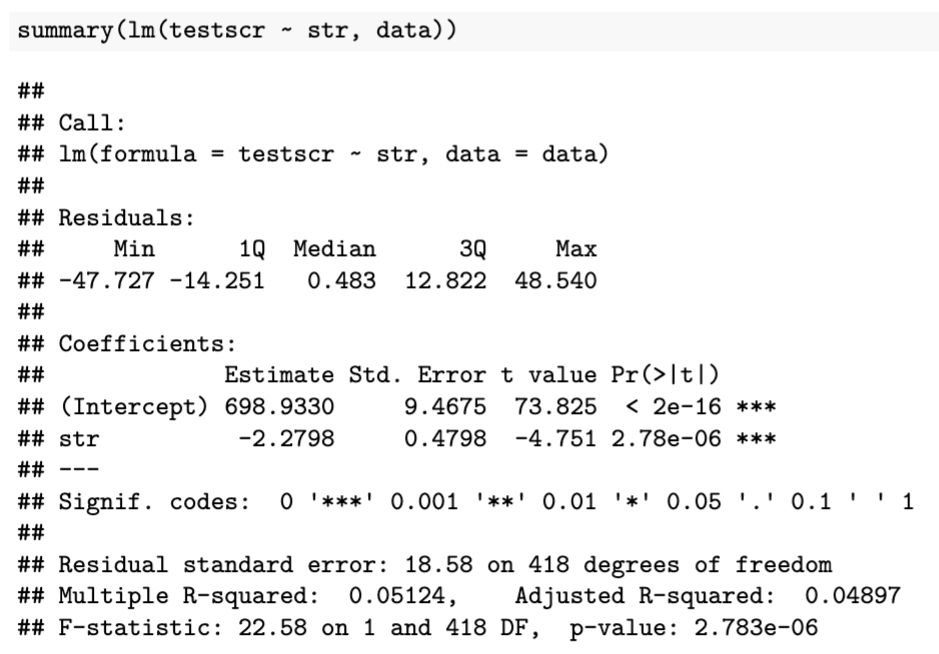
\includegraphics[scale=0.4]{reg_output.png}
\end{frame}

%%%%%%%%%%%% 
\begin{frame}{Hypothesis Testing}
From the output we can see that,
$$ \hat{\beta_1}=-2.28  \quad \text{and} \quad SE(\hat{\beta}_1)=0.48   $$ \\
In which case, the t-statistic:
$$ t = \frac{\hat{\beta_1}}{SE(\hat{\beta_1})} = \frac{-2.28}{0.48} = -4.75 $$
\vspace{0.5em}

Since $|-4.75|>2.58$, we can say that $\hat{\beta_1}$ is statistically significant at 1\% level of significance. \\~\\
\pause Is it also significant at 5\% level of significance?
\end{frame}

%%%%%%%%%%%% 
\begin{frame}{p-Value}
The p-value is the probability of drawing an outcome as or more extreme given the null hypothesis.
$$ \text{p-value} = 2 P(Z > |t|) $$
In our example, 
$$ \text{p-value} = 2 P(Z > 4.75) = 0.00 $$
Remember if $p<\alpha$, reject the null with $\alpha \%$ level of significance. 
\end{frame}


%%%%%%%%%%%% 
\begin{frame}{Output from R using Stargazer}
\vspace{-0.5em}
\centering
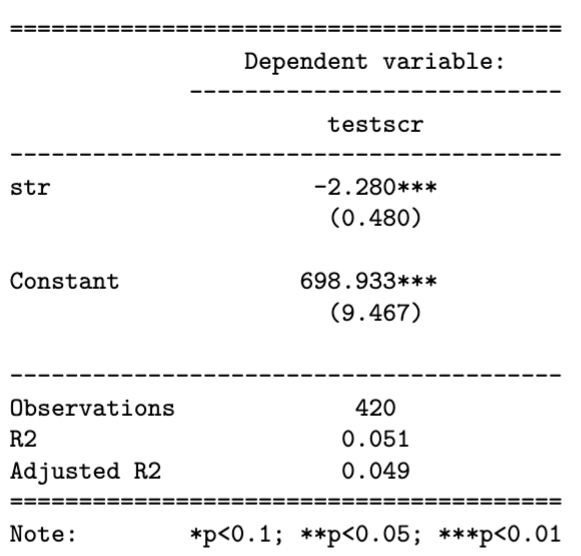
\includegraphics[scale=0.375]{reg_output_stargazer.png}
\end{frame}

%%%%%%%%%%%% 
\begin{frame}{Confidence Intervals}
As before, we can also create confidence intervals to summarize the uncertainty associated with our estimates. \\~\\
A $(1-\alpha)\%$ confidence interval for $\beta_1$:
$$ \hat{\beta}_1 \pm  z_{\alpha/2} \cdot SE(\hat{\beta}_1)  $$
If $0$ is not in the 95\% confidence interval, then once again we can say that $\beta_1$ is statistically significant at 5\% level of significance. 
\end{frame}

%%%%%%%%%%%%%%%%%%%%
\begin{frame}{Confidence Intervals}
\vfill
\centering
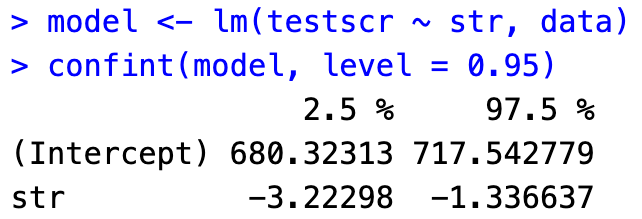
\includegraphics[scale=0.45]{ci_output.png}
\end{frame}


\end{document}